\chapter*{The first attempts}
\label{chap:The first attempts}
\renewcommand{\thesection}{\arabic{section}}
\setcounter{section}{0}

I thought that the interesting part of this project, is the simplicity and low-technicality. However the implementation turned out to be much more complex than expected. This attempt unfortunately was not accompanied with the expected success.

\section{The Android App}

The very first approach to the posture "problem" was an android App. The standard android phone offers all necessary actors and sensors and is therefore a great test environment: 
\begin{enumerate}
    \item \gls{Accelerometer} - Detects acceleration
    \item \gls{Gyroscope} - Detect orientation and angular velocity \cite{Gyroscop33:online}
    \item Vibrators
    \item Storage
\end{enumerate}

This means it was possible to get live data and calculate position and pitch in real time. Thanks to the built in vibration units, it was also possible to vibrate when a threshold was reached. With enough Android development know-how, this implementation is achievable swiftly and did work as expected.

The usability was not great and it did not feel very professional. The phone had to be held and placed near the chest or back to work. This would mean the first use case, improving the sitting position, was not achievable without holding or attaching the phone to the user and not using your phone while at work. Therefore the android app idea was quickly put aside. Since, for now at least, it does not offer what is desired.

\newpage
\section{The IoT Solution}

The next plan was to create a simple \acrshort{iot} solution (\gls{IoT}).Which I thought could be achieved by combining actors, sensors and a bit of code. However it was not as easy as expected, since the sensors and positional data is rather complex. 

The code is running on a \gls{microcontroller}, an ESP 32, specifically an ESP32 WEMOS Lolin V1.0.0. The very specific version is quite important. I will go further in depth into why, in the \textbf{difficulties}.

The \gls{ESP32} was chosen, since it offers everything you can imagine. It has a built in Bluetooth module, Wifi module and supports nearly all modern Android libraries and components. On top of that the ESP32 is cheap. It can be bought from Swiss sellers for about 10-15 CHF. It can also be imported via aliexpress.com for as low as 2-5 CH. The delivery time however, can take up to 2 months. Therefore, I considered it to be a perfect contestant for this project. 

Additionally, to the microcontroller a few more items are needed to fullfill the needed requirements. A Gyroscope, an Accelerometer, Vibrators, A Real Time Clock (\acrshort{rtc}) and a \acrshort{sd}-Card (\gls{SD}) module. The \gls{RTC} is needed since we want to log the measured values, and to analyse or visualise these logs, a time-stamp is necessary. 

All modules I have used, are used in so called breakout boards. These make the testing and development easier by offering pin-out and -in to enable swift testing. Without breakout boards the parts would be a lot smaller, however, not suitable for a first prototype since it would complicate the development process.

\subsection{The Gyroscope and Accelerometer}

After investigating, which modules are available on the market, I have decided to use the 
\gls{MPU6050} Chip since it is widely used and is documented very well. 

\begin{wrapfigure}[11]{l}{0.3\textwidth}
  \begin{center}
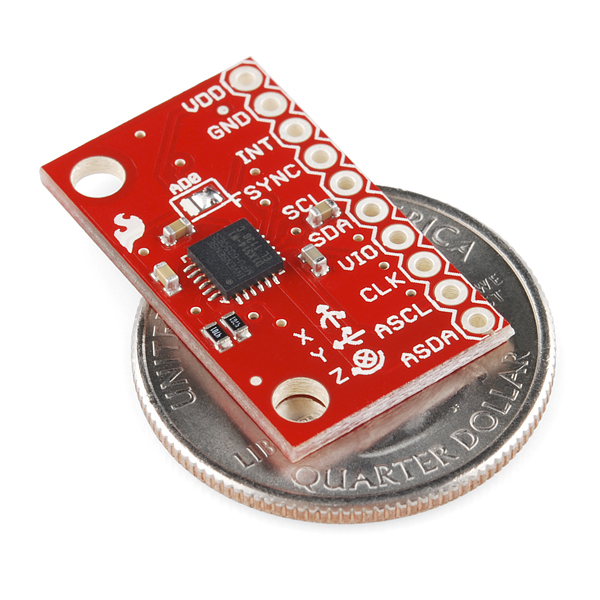
\includegraphics[width=0.3\textwidth]{images/MPU_6050.jpg}

  \end{center}
  \caption{MPU6050}
  \label{fig:MPU6050}
\end{wrapfigure}

The MPU6050 communicates via the \textbf{Wire library} and has a built in thermometer, accelerometer and gyroscope. The module is also really tiny even if it is a breakout board.
Without the breakout board this sensor would be reduced to the black square since in the picture (\ref{fig:MPU6050}).

The MPU6050 is documented very precisely which was a great help during development and made it quite easy to get the correct values. This Chip would also offer the possibility to perform some calculations directly on the Chip. Unfortunately, this part of the MPU6050 is very obfuscated. It would increase the complexity vastly without offering real benefits. This however, might be something, which will be considered in further development steps of this project.

The MPU has a very high complexity and it was quite a challenge to understand all the data, that the device provides. Especially reading the data showed to be much harder than expected. However, after some research and a lot of testing, it turned out to be much easier than firstly expected, since I was able to read the gravity which affects the accelerometer.
Currently only the values of the accelerometer are used to determine the position and sense the direction in which the user is leaning. This might be a bit to simple for the ergonomic use case, however, it is a good starting point and no technical modification are needed to get additional values.

The code for the calculation and reading of values is quite complex and really long. Therefore I will not put any code snippets in this sections since they would not provide the desired benefits to the reader. However, the whole source code will be available in my git repository. \cite{GF3RGabr46:online} \cite{TDKAttra32:online}

\newpage

\subsection{The Wire library}

To communicate with the MPU6050 and the RTC, SD Card module the wire library is necessary. With this library the communication and data exchange over only two cables (SDA Serial Data Line, SCL Serial Clock Lin) is made possible. Both modules communicate through these cables. These are located at port 21 and portvis 22 on the ESP32. The communication protocol is quite simple, and as soon as more than one device is communicating, it reduces the complexity of communication, and also soldering. Here a quick code example of the communication with the MPU6050:
\begin{lstlisting}
void readBytes(uint8_t address, uint8_t subAddress, uint8_t count, uint8_t * dest)
{  
	Wire.beginTransmission(address);   
	Wire.write(subAddress);            
	Wire.endTransmission(false);       
	uint8_t i = 0;
        Wire.requestFrom(address, count);  
        // Read bytes from slave register address 
	while (Wire.available()) {
        dest[i++] = Wire.read(); 
    }         // Put read results in the Rx buffer
}
\end{lstlisting}
\cite{MPU9250M94:online}

The communication is very well documented \cite{ArduinoW76:online} and worked on the first try. However, a difficulty definitely is and will also be, the addresses. The address of these parts is given by their manufacturer and is the same for every part. 

\subsection{The Vibrators}

Vibrators are needed to signal to the user where he should correct his position. These are, technically speaking, very basic, there is a ground and a power input, that's it. In the code, the communication therefore is also not complicated. 
I have created an enum with which, the port of the vibrators is defined:
\begin{lstlisting}
  enum VIBROPIN {
  LEFT = 16,
  RIGHT = 4,
  FORWARD = 2,
  BACKWARD = 17
};
\end{lstlisting}
Then the vibration can be triggered by simply using the keyword:
\begin{lstlisting}
 digitalWrite(RIGHT, HIGH);
\end{lstlisting}

Even though the technical implementation was manageable, the sensors are physically very fragile and definitely a week point of the build. They are very cheap and also replaceable, however, soldering them every time is quite time consuming. Therefore a work around will need to be found. Maybe these vibrators might be exchanged by led's during the development process, since that would be easier to debug and more stable. Additionally, it would provide a nice way to demonstrate the functionality. 


\subsection{SD Card}

The SD Card reader and RTC module are in the same module which makes it a bit of a special case. This might be an issue in the future since it appears to be discontinued. However, it simplified the connecting of the two modules. Therefore I will still look at them individually. 

To access the SD card module, the module "SD.h" was needed. It simplifies any file access drastically. The initialising is as follows:

\begin{lstlisting}
if(!SD.begin()){
        Serial.println("Card Mount Failed");
        return;
}
uint8_t cardType = SD.cardType();
if(cardType == CARD_NONE){
    Serial.println("No SD card attached");
    return;
}

Serial.print("SD Card Type: ");
if(cardType == CARD_MMC){
    Serial.println("MMC");
} else if(cardType == CARD_SD){
    Serial.println("SDSC");
} else if(cardType == CARD_SDHC){
    Serial.println("SDHC");
} else {
    Serial.println("UNKNOWN");
}

uint64_t cardSize = SD.cardSize() / (1024 * 1024);
Serial.printf("SD Card Size: %lluMB\n", cardSize);
\end{lstlisting}
\cite{BlogofWe42:online}

To append data to a file a helper function is used which interacts a File object which is defined in "FS.h". It enables a way to interact with different kinds of files and even create, delete or move folders and files.

\begin{lstlisting}
void appendFile(fs::FS &fs, const char * path, const char * message){
    File file = fs.open(path, FILE_APPEND);
    if(!file){
        Serial.println("Failed to open file for appending");
        return;
    }
    if(!file.print(message)){
        Serial.println("Append failed");
    }
    file.close();
}
\end{lstlisting}
\cite{BlogofWe42:online}
this function is used in the main loop to append the recorded data by the MPU to the file: 
\begin{lstlisting}
result = **all accelometerdata** + **current time**
Serial.println(result);
result.toCharArray(charBuf, 150);
appendFile(SD, "/data.txt", charBuf);
appendFile(SD, "/data.txt", "\n");
\end{lstlisting}


\subsection{Real Time Clock}

The communication with the RTC also happens via the "Wire.h" library. Furthermore, the Timelib library is needed which defines the structure tmElements\_t. This simplifies the reading of the RTC but would not be necessary. To get the time, such a tmElements\_t is passed which gets filled:
\begin{lstlisting}
bool read(tmElements_t &tm)
{
  uint8_t sec;
  Wire.beginTransmission(DS1307_CTRL_ID);
  Wire.write((uint8_t)0x00); 
  if (Wire.endTransmission() != 0) {
    exists = false;
    return false;
  }
  exists = true;

  // request the 7 data fields   (secs, min, hr, dow, date, mth, yr)
  Wire.requestFrom(DS1307_CTRL_ID, tmNbrFields);
  if (Wire.available() < tmNbrFields) return false;
  sec = Wire.read();
  tm.Second = bcd2dec(sec & 0x7f);   
  tm.Minute = bcd2dec(Wire.read() );
  tm.Hour =   bcd2dec(Wire.read() & 0x3f);  // mask assumes 24hr clock
  tm.Wday = bcd2dec(Wire.read() );
  tm.Day = bcd2dec(Wire.read() );
  tm.Month = bcd2dec(Wire.read() );
  tm.Year = y2kYearToTm((bcd2dec(Wire.read())));

  if (sec & 0x80) return false; // clock is halted
  return true;
}
\end{lstlisting}
\cite{DS1307RT51:online}

This function is used to get the current time. There is also a function which sets the time, which is necessary in a first run the have the correct time. This time is needed to create a useful log of the MPU6050 data.

\subsection{Difficulties}

During the technical implementation a few difficulties arose. The biggest one, which nearly killed the whole project, was the wire library. Especially the fix addresses. As luck, or the manufacturers, decided, both the SD Card module and the MPU6050 have the exact same adores \textbf{0x68}. This meant, that communicating while both devices were connected could not work, or at least not reliable. At the moment of realisation, many ideas came to my head, most of them are hacky and ugly. I started researching, googling and investigating. I was sure I could not have been the first one with such an issue. After about an hour of freaking out, I have found a nice solution. 
The MPU6050 offers the possibility of changing the address from 0x68 to 0x69. This can be achieved by simply connecting the AD0 port of the MPU to a "High" or 5V input.

Another bigger issue was the specific hardware I used, without knowing it. My Development board was, as mentioned ESP32 WEMOS Lolin V1.0.0. I used this board more by accident, since I did not investigate into the differences of ESP32 micro-controllers. This was only realised, when I ordered additional parts to create a "final" proof of concept (POC). The special properties of the Lolin v1.0.0 is that it provides a 5v output, which is needed by the SD card module. A standard ESP32 microcontroller only provides a 3.3v output. There would be way to route the power source separately from the ESP32, however, this was not a feasible change in the last four weeks of the project. Luckily a swiss reseller, hat the right parts which were delivery within three to four days and saved the day.
\newpage
\section{Results}

\begin{wrapfigure}[20]{R}{0.14\textwidth}
\centering
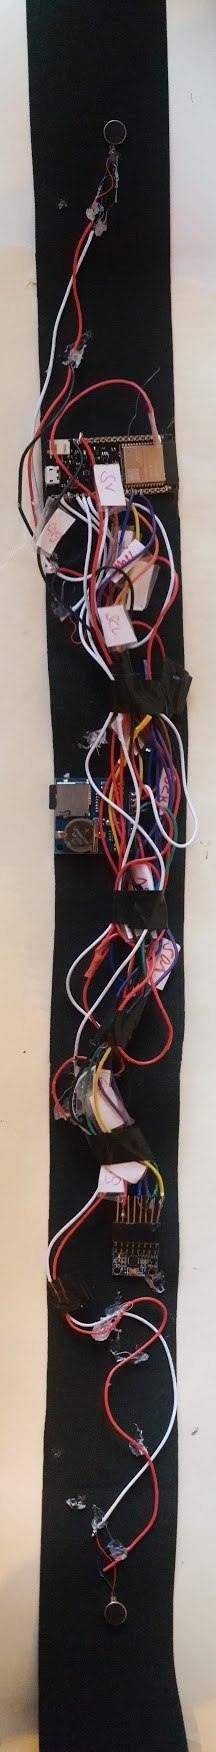
\includegraphics[width=0.14\textwidth]{images/belt.jpg}
    \caption{Belt}
        \label{fig:Belt}
\end{wrapfigure}

After these first attempts I created a simple proof of concept, which is able to read the MPU Data and interpret it to a degree, where I can tell in what direction the user is leaning. So to say, if the broom has fallen or not. This is achieved by simply reading out the accelerometer data and determining the exact position. furthermore, at the beginning of each power-on phase, a baseline reading is done to see the difference in orientation. This baseline reading currently contains of the first second of data. Then a threshold is defined, which is currently defined as follows:

\begin{lstlisting}
 if(baseZacc - (az * 1000) < -150){
       Serial.println("LEANING BACKWARD");
      digitalWrite(BACKWARD, HIGH);
    }else if(baseZacc - az * 1000 > 150){
      Serial.println("LEANING FORWARD");
      digitalWrite(FORWARD, HIGH);
    }
    if(baseYacc - ay * 1000 > 100){
       Serial.println("LEANING RIGHT");
     digitalWrite(RIGHT, HIGH);

    }else if(baseYacc - ay * 1000 < -100){
      
      Serial.println("LEANING LEFT");
      digitalWrite(LEFT, HIGH);
     }
\end{lstlisting}

The baseZacc, baseYacc and baseXacc are the values which was are read in the first second. 

Furthermore, there are four vibrators which vibrate in the direction the "broom is falling", so front, back, left or right. Additionally, the data is also recorded into an SD Card with a time-stamp. All these individual parts are soldered together and fitted into a belt which can be worn, which is displayed in the picture on the right.

The power-source still is outside of the belt, in the form of a \gls{lipo battery} which is simply connected via a micro usb cable.

The data collected has will need to be analysed in-depth. Furthermore, it appears that one single sensor does not offer the needed results or precision to detect posture. The current posture model lacks a lot of information and does not have the quality to give useful information. 

\section{Learnings}

After this first attempts I quickly realised, that connecting all the sensors via cable limited me drastically due to the restrictions of the Wire.h library and the I2C protocol. Due to the addressing issues with the current configuration, some sort of multiplexer, or custom created accelerometers and gyroscopes is needed. Custom parts would currently be way to complicated and multiplexers add unnecessary complexity to the project, I have been looking for another solution. The solution should enable me to scale up the number sensors without back-draws.

Furthermore, the current cable management and hardware complexity will need to be simplified. The current build is much higher than desired and will need to be simplified. Especially since it should be reproductionable.

